\documentclass[language=german,style=solution]{smo}

\examdate{11./12. März 2016}
\title{SMO - Finalrunde (Musterlösung)}
\examplace{1./2. Prüfung }

\begin{document}

\begin{enumerate}[label=\textbf{\arabic*.}]

%1
\item
Sei $ABC$ ein Dreieck mit $\angle BAC=60^\circ$. Sei $E$ der Punkt auf der Seite $BC$, sodass $2 \angle BAE=\angle ACB$ gilt. Sei $D$ der zweite Schnittpunkt von $AB$ und dem Umkreis des Dreiecks $AEC$ und sei $P$ der zweite Schnittpunkt von $CD$ und dem Umkreis des Dreiecks $DBE$.
Berechne den Winkel $\angle BAP$.

\textbf{Lösung:} Sei Winkel $\angle EAB=\gamma$. Da $\angle EAB = \angle DCE$ ist, liegen die vier Punkte $A$, $D$, $E$ und $C$ auf einem Kreis. Somit gilt $60^\circ-\gamma = \angle CAE=\angle CDE = \angle PDE=\angle PBE$, wobei die letzte Gleichheit wegen Sehnenviereck $DBEP$ gilt. In Dreieck $ABC$ berechnet man $\angle ABP=180^\circ -60^\circ -2\gamma-(60^\circ-\gamma)=60^\circ -\gamma$. Somit ist $BP$ die Winkelhalbierende von $\angle ABC$. Es folgt, dass $P$ der Inkreismittelpunkt von Dreieck $ABC$ ist und somit $\angle BAP=30^\circ$.
	
\includegraphics{geometrie_1_finalrunde_16_zwei}

\textbf{Marking Scheme:}
\begin{itemize}
\item  +2 $D$ liegt auf Winkelhalbierenden.
\item +2 $BP$ ist Winkelhalbierende.
\item +1 $P$ ist Schnittpunkt von Winkelhalbierenden.
\item +2 Wenn $P$ auf den Winkelhalbierenden liegt, sind wir fertig.
\item -1 $30^\circ$ nicht ausgerechnet. 
\end{itemize}
	
\newpage

%2
\item
Seien $a,b$ und $c$ die Seiten eines Dreiecks, das heisst: $a+b > c,\, b+c > a$ und $c+a > b$.\\
Zeige, dass gilt: 
\[
\frac{ab+1}{a^2+ca+1}+\frac{bc+1}{b^2+ab+1}+\frac{ca+1}{c^2+bc+1}>\frac{3}{2}.
\]

\textbf{Lösung:} Jeder der drei Summanden kann wie folgt umgeformt werden:
\[
\frac{ac+1}{c^2+bc+1}=1-\frac{c(b+c-a)}{c^2+bc+1}>1-\frac{c(b+c-a)}{c^2+bc}=\frac{a}{b+c}.
\]
Die Ungleichung gilt, da $a$, $b$ und $c$ die Seiten eines Dreiecks sind, also insbesondere positiv und $b+c-a>0$. Nesbitt liefert das gewünschte Resultat.

\textbf{Marking Scheme:}
\begin{itemize}
\item +3 Verwendung Dreiecksseiten zur (strikten) Abschätzung gegen unten des Bruchs ($1$ aus Zähler und Nenner raus)
\item +1 in Nesbitt-Form bringen (+2 falls mit Lösung)
\item 7 Lösung abschliessen.
\item 1 Richtige Strategie
\item 2 Streichen der $1$ ohne Begründung + Lösung
\end{itemize}


\newpage

%3
\item
Finde alle natürlichen Zahlen $n$, für welche Primzahlen $p,q$ existieren, sodass gilt:
\[
p(p + 1) + q(q +1) = n(n + 1).
\]
\textbf{Lösung:} Wir ziehen $q(q+1)$ von beiden Seiten der Gleichung ab. Faktorisieren liefert
\[
p(p+1)=(n-q)(n+q+1).
\]
Falls $p$ ein Teiler von $n-q$ ist, gibt es keine Lösung, da $p+1$ dann kleiner als $n+q+1$ ist. Somit teilt $p$ den Term $n+q+1$. Analog zur obigen Faktorisierung bekommen wir, dass $q$ ein Teiler von $n+p+1$ ist. Zuerst betrachten wir die Möglichkeit $p=q$.  Dann gilt $2p(p+1)=n(n+1)$. $p$ teilt $n+1$. Somit ist $p+1$ ein Teiler von $n$ und folglich $2$ ein Teiler von $n+1$. Es folgt $2(n+1)=p$ und $p=n$, also $p=2$. Dies gibt uns die Lösung $(p,q,n)=(2,2,3)$.
	
Nun können wir annehmen, dass $p$ grösser als $q$ ist. Somit ist $p$ grösser als $n/2-1$. Ausserdem ist $q$ kleiner als $n$. Daraus folgt, dass wir die drei Fälle $p=n+q+1$, $2p=n+q+1$ und $3p=n+q+1$ betrachten müssen. Im ersten Fall gibt es keine Lösung, da $p$ kleiner als $n$ ist. Im zweiten Fall bekommen wir mit $2p-n-1=q$ und $q \mid n+p+1$, dass $q$ ein Teiler von $3p$ ist. Da $p$ grösser als $q$ ist, bleibt die Möglichkeit $q=3$. Einsetzen von $q=3$ und $n=2p-4$ liefert die quadratische Gleichung $3p^2-15p=0$ und somit die Lösung $(p,q,n)=(3,5,6)$. Im dritten Fall bekommen wir mit $3p-n-1=q$ und $q\mid n+p+1$, dass $q$ ein Teiler von $4p$ ist. Da $p$ grösser als $q$ ist, bleibt der Fall $q=2$. Einsetzen von $n=3p-3$ liefert, dass $p(8p-16)=0$ ist. Die linke Seite ist aber für $p>q=2$ strikt positiv, also bekommen wir in diesem Fall keine Lösung.
	
Somit sind $(2,2,3)$ und $(3,5,6)$ die beiden einzigen Lösungen.

\textbf{Marking Scheme:}
\begin{itemize}
\item +2 nützliche Faktorisierung
\item +1 Fallunterscheidung
\item +1 Abschätzung $2p \geq n$
\item 7 für den Rest
\item -1 für vergessene Fälle
\end{itemize}

\newpage

%4
\item On considère 2016 points distincts dans le plan. Montrer qu'on peut trouver au moins $45$ distances différentes entre ces points.

\textbf{Solution:} 	Soit $E$ l'enveloppe convexe des $2016$ points (le plus petit ensemble convexe qui contient tous les points) et soit $P$ un point de notre ensemble qui est sur le bord de $E$. Si depuis $P$ il y a au moins $45$ distances, l'exercice est prouvé.
	
	Sinon on peut tracer $44$ cercles centrés en $P$ de telle manière que tous les points autres que $P$ soient situés sur un de ces cercles. Comme $44\cdot 45 = 1980 < 2016$, il existe un cercle $\Gamma$ qui contient au moins $46$ points de notre ensemble. De plus, comme $P$ est sur le bord de l'enveloppe convexe $E$, l'intersection des cercles avec $E$ donne au plus un demi-cercle.
	
	On choisit donc sur $\Gamma$ un des deux points les plus à l'extrémité de l'arc de cercle, et on appellera ce point $Q$. Comme il y a au moins $46$ points sur $\Gamma$ il suffit de montrer que $Q$ a une distance différente avec tous les points de $\Gamma$ pour pouvoir conclure qu'on a bien au moins $45$ distances. Or, cette dernière affirmation est vraie car la partie de $\Gamma$ qui est contenue dans $E$ est au plus un demi-cercle et comme $Q$ a été choisi à l'extrémité de cet arc de cercle, si deux points de $\Gamma$ avaient la même distance à $Q$ ils devraient se trouver de part et d'autre du diamètre passant par $Q$, ce qui est impossible.
	
	On a donc bien au moins $45$ distances.
	
\textbf{Marking Scheme:}
\begin{itemize}
\item +1 46 Punkte auf einem Kreis zeigen.
\item +2 Betrachtung eines Punktes auf der konvexen Hülle beziehungsweise die Beiden mit dem grössten Abstand und zeigen, dass alle Punkte auf Halbkreisen liegen.
\item +2 wenn man beide zusammen hat.
\item 7 Lösung beenden. (45 Distanzen auf einem Halbkreis mit 46 Punkten)
\end{itemize}

\newpage

%5
\item Sei $ABC$ ein rechtwinkliges Dreieck mit $\angle ACB = 90^\circ$ und $M$ der Mittelpunkt von $AB$. Sei $G$ ein beliebiger Punkt auf der Strecke $MC$ und $P$ ein Punkt auf der Geraden $AG$, sodass $\angle CPA = \angle BAC$ gilt. Weiter sei $Q$ ein Punkt auf der Geraden $BG$, sodass $\angle BQC = \angle CBA$ gilt. Zeige, dass sich die Umkreise der Dreiecke $AQG$ und $BPG$ auf der Strecke $AB$ schneiden.

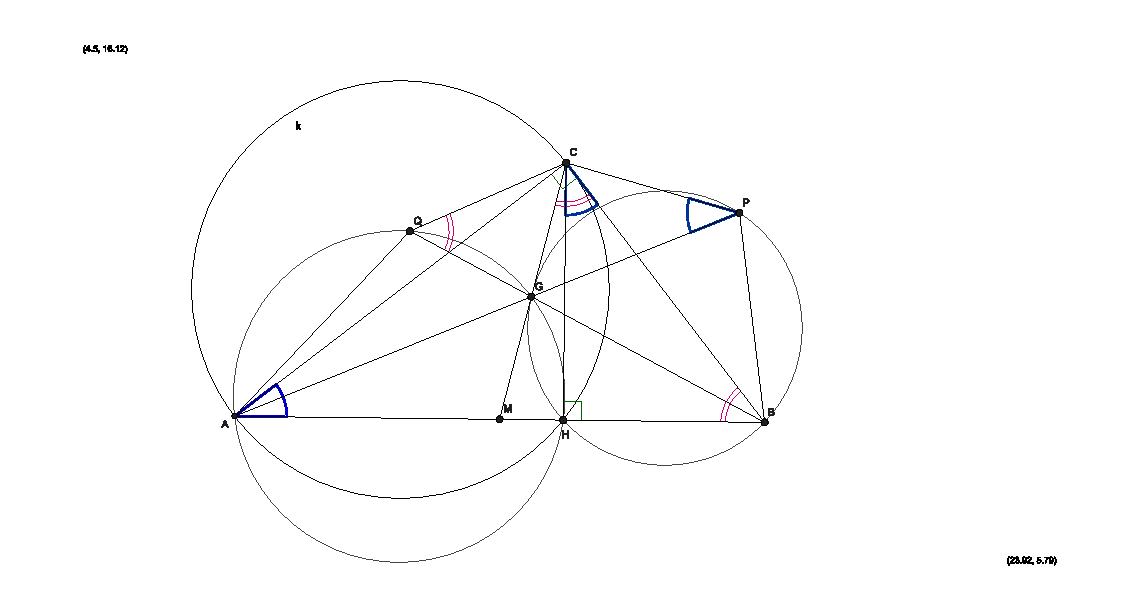
\includegraphics{finalrunde_5_2016.pdf}

\textbf{Lösung:} Sei $H$ der Höhenfusspunkt von $C$. Wir wollen zeigen, dass der Umkreis vom Dreieck $AGQ$ die Strecke $AB$ in $H$ schneidet.\\
Simple Winkeljagd liefert, dass $\angle BAC = \angle HBC$. Mit der Umkehrung des Tangentenwinkelsatzes folgt, dass die Gerade $BC$ tangential an den Umkreis $k$ vom Dreieck $AHC$ ist. Nun erhält man mit der Potenz von $B$ an $k$, dass gilt:
\[
BA \cdot BH = BC^{2}
\]
Weiter ist M der Umkreismittelpunkt vom Dreieck $ABC$ und somit ist das Dreieck $CMB$ gleichschenklig. Daraus folgt, dass $\angle BQC = \angle CBA = \angle MCB$. Mit der Umkehrung des Tangentenwinkelsatzes und der Potenz von $B$ an den Umkreis vom Dreieck $CQG$ erhält man:
\[
BQ \cdot BG = BC^{2}
\]
Aus diesen beiden Gleichungen folgt:
\[
BA \cdot BH = BQ \cdot BG
\] 
Mit der Potenz von $B$ an den Umkreis vom Dreieck $AGQ$ folgt, dass $H$ auch auf dem Umkreis liegt.\\
Auf ähnliche Weise folgt, dass $H$ auf dem Umkreis vom Dreieck $BPG$ liegt. Und somit schneiden sich die beiden Umkreise auf $AB$.

\textbf{Marking Scheme:} 
\begin{itemize}
\item $BC$ tangent an $QGC$ oder $AC$ tangent an $GPC$ 2P
\item $BC$ tangent an $AHC$ oder $AC$ tangent an $BCH$ 2P
\item Fertig machen 3P
\end{itemize}

\newpage

%6
\item Sei $a_n$ eine Folge natürlicher Zahlen definiert durch $a_1 = m$ und $a_n = a^2_{n-1}+1$ für $n>1$. Ein Paar $(a_k, a_l)$ nennen wir \emph{interessant}, falls
\begin{enumerate}[(i)]
\item $0<l-k<2016$,
\item $a_k$ teilt $a_l$.
\end{enumerate}
Zeige, dass ein $m$ existiert, sodass die Folge $a_n$ kein interessantes Paar enthält.

\textbf{Lösung:} Die zweite Bedingung ist genau dann erfüllt, wenn $a_l$ kongruent zu 0 modulo $a_k$ ist. Schauen wir also die möglichen Resultate von $a_l$ modulo $a_k$ an.
Für $l=k+1,k+2$ berechnen wir:
\begin{align*}
a_{k+1} = a_k ^2 + 1 \equiv 1 \pod{a_k}\\
 a_{k+2} = a_{k+1} ^2 + 1 \equiv 1 + 1 = 2 \pod{a_k}
 \end{align*}
Wenn wir so weiterfahren bis $l=k+2015$ erhalten wir 2015 solcher Zahlen. Zu bemerken ist, dass keine dieser Zahlen von $a_k$ abhängt. Sei $M$ das Maximum dieser Zahlen. Damit wir nie $a_l$ kongruent zu null modulo $a_k$ erhalten, reicht es sicherzustellen, dass $a_k$ strickt grösser ist als $M$.
Weiter haben wir durch die Rekursionsformel, dass $a_k < a_{k+1}$ und somit, $m < a_k$ für jedes $k$. Das heisst, wenn wir $m$ grösser als $M$ wählen, ist auch $a_k$ grösser als $M$. Wir können also folgern, dass es kein interessantens Paar gibt.

\textbf{Marking Scheme:}
\begin{itemize}
\item Betrachtung mod $a_k$ 1P
\item Alle Reste sind gleich 2P
\item $m > rest_{2016}$ Einsetzen 2P
\item Fertig	 2P
\end{itemize}

\newpage

%7
\item Auf einem Kreis liegen $2n$ verschiedene Punkte. Die Zahlen $1$ bis $2n$ werden zufällig auf diese Punkte verteilt. Jeder Punkt wird mit genau einem anderen Punkt verbunden, sodass sich keine der entstehenden Verbindungsstrecken schneiden. Verbindet eine Strecke die Zahlen $a$ und $b$, so weisen wir der Strecke den Wert $\abs{a-b}$ zu. Zeige, dass wir die Strecken so wählen können, dass die Summe dieser Werte $n^2$ ergibt.

\textbf{1. Lösung:}
Man sieht, dass $(n+(n+1)+...+2n) - (1+2+...+n) = n^2$ ist. Also falls wir es schaffen jede Zahl aus der zweiten Klammer mit einer aus der ersten Klammer (natürlich ohne Überkreuzungen) zu verbinden sind wir fertig. Es gibt immer eine Zahl aus der ersten Klammer die neben einer Zahl in der zweiten Klammer ist egal wie sie angeordnet sind. Wir verbinden ein solches Paar und schauen nur noch die $2n-2$ übrigen Punkte an. Egal welche Verbindungsstrecken wir einzeichnen, sie schneiden die weggenommene sicher nicht. Nun machen wir das Analog weiter, bis wir keine Zahlen mehr zu verbinden haben. Die Summe aller Strecken ist $n^2$ und wir haben keine Schnittpunkte. Somit sind wir fertig.

\textbf{2. Lösung:}
Wie oben sieht man die beiden Zahlengruppen. Da es nicht darauf ankommt welche aus der ersten Gruppe mit denen aus der zweiten Gruppe verbindet werden können wir sie vereinheitlichen. Die $n$ Punkte in der ersten Gruppe machen wir rot und die $n$ in der zweiten blau. Jetzt wollen wir zeigen, das wir die roten mit den blauen Punkten verbinden können ohne Schnittpunkte haben. Dazu verbinden wir sie zuerst irgendwie. Jetzt wählen wir einen beliebigen Schnittpunkt und tauschen die beiden Verbindungen so, dass blau wieder mit rot verbunden ist. Somit haben wir einen Schnittpunkt weniger. Denn es entstehen keine neuen Schnittpunkte, da jede Strecke eine der beiden neuen Strecken schneidet schon eine alte schneidet, denn beide neuen Strecken bilden mit je zwei der alten Teilstrecken ein Dreieck. Und jede Strecke die in eines der Dreiecke hinein geht muss auch wieder hinausgehen, da kein Punkt des Kreises im Dreieck liegt.

\textbf{Marking Scheme:}
\begin{itemize}
\item +1 Séparer les nombres en deux groupes: $[1, \dots, n]$ et $[n+1, \dots, 2n]$\\
\item Première solution:
\begin{itemize}[$\triangle$]
\item +2 Il existe deux points qui appartiennent respectivement aux deux groupes côte à côte
\item +2 Montrer qu'on peut les relier et les ignorer par la suite
\item +2 Terminer
\end{itemize}
\item Deuxième solution:
\begin{itemize}[$\triangle$]
\item +2 Si deux segments s'intersectent, les échanger de manière à toujours relier un bleu à un rouge
\item +3 Montrer que le nombre d'intersections par ce processus devient strictement plus petit
\item +1 Terminer
\end{itemize}
\item -1 Si en utilisant les longueurs des segments dans la deuxième solution on prouve que la somme des longueurs diminue mais on ne dit pas qu'il existe un nombre fini de configurations possible
\item -1 Si dans la première solution on ne justifie pas qu'il existe deux points des deux groupes côte à côte
\end{itemize}

\newpage

%8
\item Soit $ABC$ un triangle aigu et soit $H$ son orthocentre. Soit $G$ l'intersection de la parallèle à $AB$ passant par $H$ avec la parallèle à $AH$ passant par $B$. Soit $I$ le point sur la droite $GH$ tel que $AC$ coupe le segment $HI$ en son milieu. Soit $J$ la deuxième intersection de $AC$ avec le cercle circonscrit au triangle $CGI$. Montrer que $IJ=AH$.

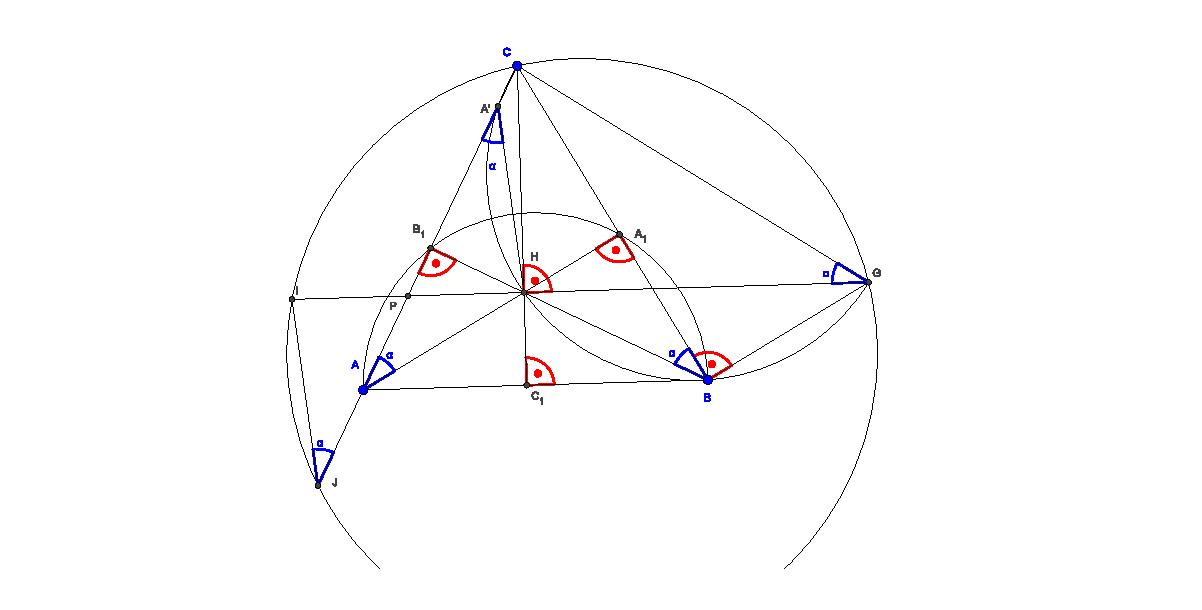
\includegraphics{finalrunde_8_2016.pdf}

\textbf{Solution:}
Soient $A_1,B_1$ et $C_1$ les pieds des hauteurs passant respectivement par $A,B$ et $C$ et soit $P$ le point d'intersection de $AC$ avec $GI$. Nous montrons d'abord que les deux quadrilatères $CHBG$ et $BA_1B_1A$ sont des quadrilatères inscrits.
	
En effet, puisque $H$ est l'orthocentre du triangle $\triangle ABC$, que $HG$ est parallèle à $AB$ et que $BG$ est parallèle à $AH$ nous avons 
\[
\angle CHG = \angle CC_1B = 90^{\circ} = \angle AA_1B = \angle A_1BG = \angle CBG
\]
donc $CHBG$ est inscrit. On voit aussi facilement que $\angle AA_1B = 90^{\circ} = \angle AB_1B$ donc $BA_1B_1A$ est aussi un quadrilatère inscrit. 
	
Puisque par construction $GCIJ$ est également un quadrilatère inscrit, nous avons alors 
\[
\angle IJC = \angle IGC = \angle HGC = \angle HBC = \angle B_1BA_1 = \angle B_1AA_1 = \angle CAH
\]
On introduit alors le point $A'$ sur la droite $AC$ tel que $HA = HA'$. Comme $AHA'$ est isocèle nous avons alors 
\[
\angle PA'H = \angle AA'H = \angle A'AH = \angle CAH = \angle IJC = \angle IJP
\]
D'autre part, nous avons aussi $\angle HPA' = \angle IPJ$ car ils sont opposés par le sommet. Ainsi, puisque $IP = HP$, les deux triangles $\triangle IJP$ et $\triangle HA'P$ sont égaux, donc $IJ = A'H = AH$.

\textbf{Marking Scheme:}
\begin{itemize}
\item $CHBG$ ist ein Sehnenviereck 2P
\item $\angle IJC=\angle CAH$ 2P
\item Wichtiges Objekt finden 2P
\item Fertig	 1P
\end{itemize}

\newpage

%9
\item Soit $n \geq 2$ un nombre naturel. Pour un sous-ensemble $F$ à $n$ éléments de $\{1, \ldots, 2n\}$, on définit $m(F)$ comme le minimum de tous les $\kgV{(x,y)}$, où $x$ et $y$ sont deux éléments distincts de $F$. Trouver la valeur maximale que peut atteindre $m(F)$.

\textbf{Solution:} Nous montrons d'abord que $m(F)$ atteint son maximum pour $F = \{n+1, \ldots, 2n\}$. En effet soit $G$ un autre sous-ensemble et $x \leq n$ un élément de $G$.
\begin{enumerate}
\item Si $2x$ est aussi un élément de $G$, alors $m(G) \leq \kgV{(x, 2x)} = 2x$. D'autre part comme tout élément de $F$ est strictement supérieur à $n$, aucun ne divise un autre et donc pour toute paire $x\neq y$ d'éléments de $F$, $\kgV{(x, y)} > 2n$, donc $m(F) > m(G)$.
\item Si $2x$ n'est pas un élément de $G$, pour tout $y\neq x$ élément de $G$, nous avons $\kgV{(x, y)} \leq \kgV{(2x, y)}$ donc si $G'$ est l'ensemble obtenu à partir de $G$ en remplaçant $x$ par $2x$, on a alors que $m(G) \leq m(G')$
\end{enumerate}
Le maximum est donc atteint quand $G$ n'a aucun élément parmi $\{1,\ldots, n\}$, c'est-à-dire quand $G = F$ (même s'il peut aussi être atteint pour d'autres ensembles $G$).
			
Il suffit donc de calculer $m(F)$ pour $F = \{n+1, \ldots, 2n\}$. Soient donc $x_0 < y_0$ des éléments de $F$ tels que $m(F) = \kgV{(x_0, y_0)}$. Si $d = \ggT{(x_0, y_0)}$, on a alors que $m(F) = \frac{x_0\cdot y_0}{d}$.
Or, comme $y_0 = x_0 + k\cdot d$ pour un certain $k\in \N$ et que $(x_0, y_0)$ minimisent $\kgV{(x_0, y_0)} = \frac{x_0\cdot y_0}{d}$, on a forcément $k=1$, donc $m(F) = x_0\cdot\left(\frac{x_0}{d}+1\right)$.
	
On commence par calculer que pour $n \leq 4$, $m(F)$ vaut successivement $12, 12$ et $24$. Maintenant pour $n\geq 5$, on traite séparément $n$ pair et $n$ impair:
\begin{itemize}
\item Si $n$ est impair, pour $x_0 = n+1$ et $d = \frac{n+1}{2}$, on obtient $y_0 = \frac{3(n+1)}{2}$ et comme $x_0$ est le plus petit élément de $F$ et pour n'importe quel choix de $x_0$ dans $F$ $\frac{x_0}{d} \geq 2$, on a que $m(F) = \kgV{(x_0, y_0)} = 3(n+1)$. De plus $y_0 = \frac{3(n+1)}{2} \leq 2n$ car cette inéquation est équivalente à $n\geq 3$, qui est vraie puisqu'on considère $n\geq 5$.
\item Si $n$ est pair, pour $x_0 = n+2$ et $d = \frac{n+2}{2}$, on obtient $y_0 = \frac{3(n+2)}{2}$. Comme $\frac{x_0}{d} = 2$, le seul autre candidat pour $x_0$ serait $n+1$ mais comme $n+1$ est impair nous aurions alors $\frac{x_0}{d'} \geq 3$, donc $(n+1)\cdot\left(\frac{n+1}{d'}+1\right) \geq (n+1)\cdot 4 \geq (n+2)\cdot 3 = (n+2)\cdot\left(\frac{n+2}{d}+1\right)$ car cette inéquation est équivalente à $n\geq 2$. On a donc que $m(F) = \kgV{(x_0, y_0)} = 3(n+2)$. Enfin on constate que $y_0 = \frac{3(n+2)}{2} \leq 2n$ car l'inéquation est équivalente à $n\geq 6$.
\end{itemize}
	
La solution est donc $3(n+1)$ si $n$ est impair et $3(n+2)$ si $n$ est pair, avec comme seule exception $n=4$ où la solution est 24.

\textbf{Marking Scheme:}
\begin{itemize}
\item +1 Multiplikation mit einer Zahl macht das kgV nicht kleiner
\item +2 Zeigen, dass das Maximum mit der Menge $\{n+1,...,2n\}$ erreicht wird.
\item +1 Vermutung der maximalen Menge und der richtigen Lösung.
\item +2 Zeigen, dass das minimale kgV dieser Menge wirklich $3(n+1)$ (ungerade) beziehungsweise $3(n+2)$ ist.
\item 7 Lösung beenden.
\end{itemize}

\newpage

%10
\item Finde alle Funktionen $f\colon\R\to\R$, sodass für alle $x,y\in\R$ gilt:
\[
f(x+yf(x+y))=y^2+f(xf(y+1)).
\]

\textbf{Lösung:}
Setze $y = 0$, um
\begin{equation}\label{funktionalgleichung1}
f(x) = f(xf(1))
\end{equation}
zu erhalten. Setze nun $x = 0$:
\begin{equation}\label{funktionalgleichung2}
f(yf(y)) = y^2 + f(0).
\end{equation}
Es folgt
\[
y^2 + f(0) =^{(2)} f(yf(y)) = f(yf(1)f(yf(1))) = (yf(1))^2 + f(0).
\]
Setze darin $y = 1$ um $f(1)^2 =  1$ zu erhalten. Wir unterscheiden zwei Fälle: \\
Fall 1: $f(1) = -1$ \\
Aus \eqref{funktionalgleichung1} folgt sofort, dass $f$ gerade ist. Setze nun $x = y = -\frac{1}{2}$ in der Originalgleichung: \\
$f( -\frac{1}{2}  -\frac{1}{2}f(-1)) = \frac{1}{4} + f( -\frac{1}{2}f( \frac{1}{2})) \Leftrightarrow
f( -\frac{1}{2}  -\frac{1}{2}f(1)) = \frac{1}{4} + f( \frac{1}{2}f( \frac{1}{2})) \Leftrightarrow f(0) = \frac{1}{2} + f(0),$ ein Widerspruch. Dabei haben wir zuerst die Geradheit von $f$ verwendet und dann (2). \\
Fall 2: $f(1) = 1$ \\
Setze $y = 1$ in \eqref{funktionalgleichung2} um $f(0) = 0$ zu erhalten. Wir zeigen nun, dass $f$ injektiv an der Stelle 1 ist. Nimm also an, dass $a \in \R$ mit $f(a) = 1$ gilt (wir wissen bereits, dass eines existiert). Sei $y = a$ in (2): $a^2 = f(af(a)) = f(a) = 1$. Wir müssen also nur noch den Fall $f(-1) = 1$ ausschliessen. Angenommen, dass $f(-1) = 1$ gilt, führt das Einsetzen von $y = -2$ und $x = 1$ in der Originalgleichung zu einem Widerspruch: $f(1 - 2f(-1)) = 4 + f(f(-1)) \Leftrightarrow f(-1) = 4 + f(1) \Leftrightarrow 1 = 5.$ Also ist $f$ injektiv bei 1. \\
Mit $y = -1$ in der Originalgleichung folgt nun $f(x - f(x - 1)) = 1$. Mit der Injektivität impliziert dies $f(x - 1) = x - 1$, also $f(x) = x \ \forall x \in \R$.

\begin{itemize}
\item +2 $f(1)^2=1$
\item +1 $f(1)\neq -1$
\item +2 $1$ ist die einzige reelle Zahl, die auf $1$ geschickt wird.
\item 7 Lösung beenden.
\end{itemize}


\end{enumerate}

\bigskip

\vspace{1cm}

\center{\translation{Viel Glück!}{Bonne chance!}{Buona fortuna!}}

\end{document}
